% !TEX root = ../patchEmbeddings_review.tex

\begin{figure}[t]
\centering
        % \includegraphics[width=0.4\textwidth,trim=0.25in 0.25in 0.68in 0.36in,clip]{./figs/SSBM_experiments.pdf} % 0.45
        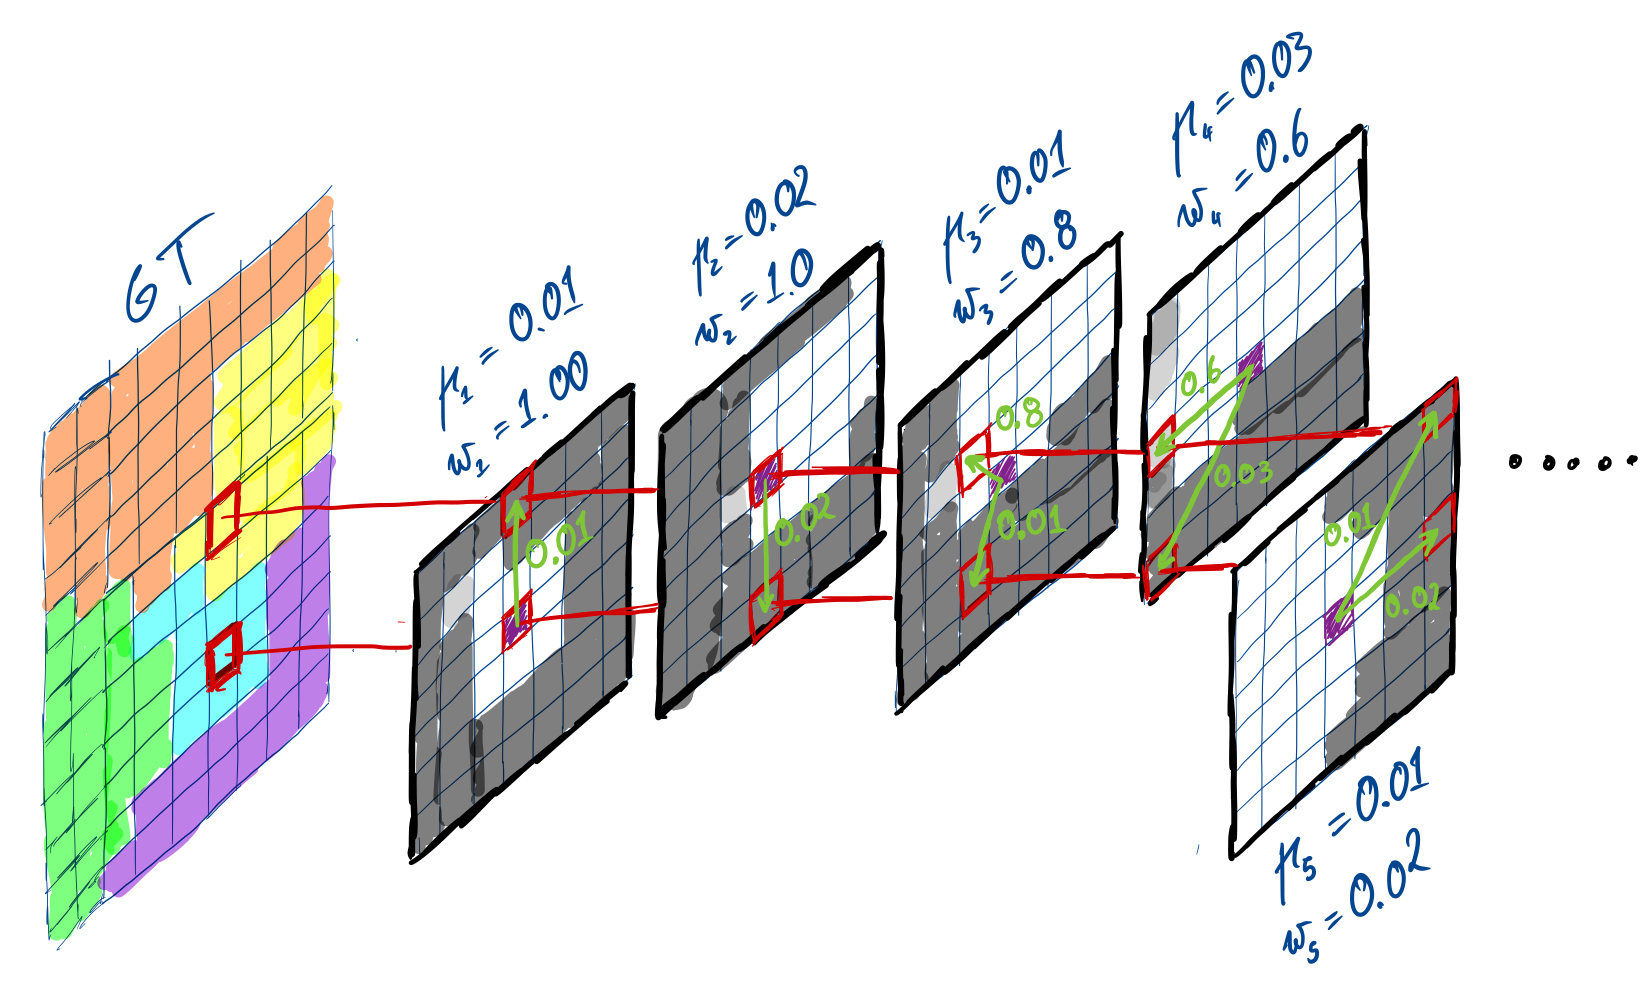
\includegraphics[width=0.7\textwidth]{./figs/alg_explaned.jpg} % 0.45
        \caption{Illustration of the proposed parameter-free method to convert \maskname masks to edge weights...}
    \label{fig:alg_explained}
\end{figure}
\begin{algorithm}[t]
  \begin{flushleft}
  \caption{: Affinities from aggregated \maskname masks}
   \hspace*{\algorithmicindent} \textbf{Input:} Graph $\mathcal{G}(V,E)$; \maskname masks $\mathcal{M}_{\coord{u}}: \mathcal{N}_{K\times K} \rightarrow [0,1]$  \\
  \hspace*{\algorithmicindent} \textbf{Output:} Affinities $\bar{a}_e\in[0,1]$ with variance $\sigma^2_e$ for all edges $e\in E$\\
  \hspace*{\algorithmicindent} 
  \begin{algorithmic}[1]
  \footnotesize
  % \small
      % \State Initial clustering: $\Pi=\{\{v_1\}, \ldots, \{v_{|V|}\}\}$
      % \State Initialize interactions between clusters with $ = w^+_e - w^-_e$
      \For{each edge $e\in E$ in graph $\mathcal{G}$}
        \State Get coordinates $\coord{u}=(u_x,u_y)$ and $\coord{v}=(v_x,v_y)$ of pixels linked by edge $e$

        % \State Init. accumulation sets $\mathcal{A}=\{\}$ for affinities and $\mathcal{W}=\{\}$ for reliability weights
        \For{each $i$-th mask $\mathcal{M}_{\coord{c}_i}$ including both pixel $\coord{u}$ and pixel $\coord{v}$}
            \State Get relative coords. of $\coord{u}$ and $\coord{v}$ with respect to the central pixel $\coord{c}_i$
            \State $a_i \gets \min \big(\mathcal{M}_{\coord{c}_i}(\coord{u} - \coord{c}_i), \,\mathcal{M}_{\coord{c}_i}(\coord{v} - \coord{c}_i)\big)$ \Comment{Fuzzy-AND: both values active}
            \State $\omega_i \gets \max \big(\mathcal{M}_{\coord{c}_i}(\coord{u} - \coord{c}_i), \,\mathcal{M}_{\coord{c}_i}(\coord{v} - \coord{c}_i)\big)$ \Comment{Fuzzy-OR: at least one value active}
        \EndFor
        \State Get weighted affinity average $\bar{a}_e= \sum_{i} a_i \omega_i\,/\,\sum_{i}\omega_i$ 
        \State Get weighted affinity variance $\sigma^2_e = \sum_{i} \omega_i (a_i-\bar{a}_e)^2\,/\,\sum_{i}\omega_i$
      \EndFor
      \State
      \Return $a_e, \sigma^2_e$ for each $e\in E$
  \end{algorithmic}
    \label{computing_affinities}
  \end{flushleft}

\end{algorithm}

\section{Extracting affinities from \maskname masks}
In this section we describe how to extract a sparse stencil of affinities from the \maskname masks predicted by our model, so that they can be used as edge weights of a pixel grid-graph. 
% Finally, a graph partitioning algorithm yields object instances.


\cite{liu2016multi} \emph{The patch pair with the highest overlap score is selected where corresponding segment masks are merged. This process iterates until no existing patch pair has the overlap score higher than a given threshold. Different scales are treated independently and duplicates are handled via non-max suppression}

\TODO{To be completed}
% A lot of recently proposed instance-segmentation methods, predict pairwise affinity between pairs of pixels 
By predicting a \maskname mask for each pixel, the pairwise affinity between two pixels is predicted 


One common used method is to predict a set of sparse affinities for every pixel (see Fig. \ref{fig:comparing_masks_affs}c)... 
These can then be see as edge weights of a grid-graph where each node represents a pixel of the image. And a graph clustering algorithm is then applied to output an instance segmentation.
In this section, we propose to ways to perform something similar and use the predicted per-pixel \maskname masks to define the edge weights of a grid-graph.
First, in Sec. \ref{sec:efficient_affs} we propose a simple way to efficiently extract a set of sparse affinities from the predicted encoded \maskname masks, without the need to decode them one by one. Then, in Sec. \ref{sec:prob_affs}...

\subsection{Efficient computation of sparse affinities from encoded masks}\label{sec:efficient_affs}
A commonly used instance segmentation method predicts, for each pixel, a small set of sparse short- and long-range affinities representing how likely it is for a pair of pixels to belong to the same object instance (see Fig. \ref{fig:comparing_masks_affs}c).



As a second contribution, we propose two distinct ways of converting the predicted per-pixel \maskname masks into edge weights of a graph representing the image, so that each node corresponds to a pixel and a graph clustering algorithm is then used to output an instance segmentation.

Here it would be nice to claim that hopefully the set of affinities we get out of this leads to more consistent neighborhood structures as compared to directly predicting each affinity as an output channel of the main model

\subsection{Averaged }\label{sec:prob_affs}
\begin{itemize}
\item Every patch predicts $M\times N$ affinities between the central pixel and the neighboring ones. But can we do better?
\item Defining the graph: we have an edge between two nodes $(i, j)$ only if $j \in M\times N$ Given two pixels  
\item training patches makes the task more difficult (than just learning a boundary prediction)
\end{itemize}
- 


The second proposed method yields a parameter-free algorithm achieving competitive performances, yada yada yada... 



